%%%%%%%%%%%%%%%%%%%%%%% file moduleX_template.tex %%%%%%%%%%%%%%%%%
%
%
% This is a template for creating your papers for the course KRW
% It is based on the standard Latex template for Springer publications
% but contains a suggestion for the structure and some content of the 
% paper. 
%
% Please adapt this document wherever needed.
%
% For more information about the required Latex Style check the document
% typeinst.pdf in the StyleFiles directory. 
%
%%%%%%%%%%%%%%%%%%%%%%%%%%%%%%%%%%%%%%%%%%%%%%%%%%%%%%%%%%%%%%%%%%%%%%%%%


\documentclass[runningheads,a4paper]{../../StyleFiles/llncs}

\usepackage{url}
\usepackage{graphicx}
\usepackage{amssymb}
\usepackage{listings}
\lstset{language=SQL,morekeywords={PREFIX,java,rdf,rdfs,url}}
 

\newcommand{\keywords}[1]{\par\addvspace\baselineskip
\noindent\keywordname\enspace\ignorespaces#1}

\begin{document}

\mainmatter  % start of an individual contribution

% first the title is needed
\title{Data- and Systems Paper : Finding Amsterdam}

% a short form should be given in case it is too long for the running head
\titlerunning{Data- and Systems Paper}

% the name(s) of the author(s) follow(s) next
%
% NB: Chinese authors should write their first names(s) in front of
% their surnames. This ensures that the names appear correctly in
% the running heads and the author index.
%
\author{Alivanistos, Dimitris. \\ Baez, Selene. \\ Jemmett, Andrea. }
%
\authorrunning{Alivanistos, Dimitris. \\ Baez, Selene. \\ Jemmett, Andrea.}
% (feature abused for this document to repeat the title also on left hand pages)

% the affiliations are given next; don't give your e-mail address
% unless you accept that it will be published
\institute{\url{d.alivanistos@student.vu.nl} \and \url{s.baezsantamaria@student.vu.nl} \and \url{a.jemmett@student.vu.nl}}

\maketitle


\begin{abstract}
The abstract should summarize the contents of the paper and should
contain at least 70 and at most 150 words. It should be written using the
\emph{abstract} environment.
\end{abstract}


\section{Introduction}
In the journey of having a Semantic Web where everything is linked, open and reusable, dealing with volume is necessary. The same way as in "Finding Wally", the tangled world of Linked Data makes it virtually impossible to find some specific information. The problem becomes even more complex when the information to be retrieved is not clear, in which case the task is comparable to fishing in the darkness.

Given the trends in the Semantic Web, it is undeniable that finding specific information, and reasoning in large heterogeneous datasets will become a need. Thus efficient mechanisms are required to achieve these goals. In fact, this year's \textit{International Semantic Web Conference} \footnote{\url{http://iswc2016.semanticweb.org/pages/calls/research-track.html}}, held in Kobe, Japan, recognizes it as one of the main topics of interest, phrasing it as "Architectures and algorithms for extreme volume, heterogeneity, dynamicity, and decentralization of Semantic Web data"

In this paper we address the previous challenge with approximation techniques as a tool for efficient reasoning over a large dataset. To link this to our previous work, we select the specific domain of Amsterdam, and aim to retrieve all the Amsterdam-related information from the provided \texttt{dataset} in Stardog.  

The goal of this assignment is to compare two approximation techniques. On the one hand, we randomly choose a subset of nodes, and retrieve all information related to Amsterdam. On the other hand, we do a smarter selection of nodes and repeat the process. We hypothesize the "smart selection" approach will have higher accuracy than the "random" approach on approximating the original set. Yet, smart selection requires statistical analysis and reasoning over the set, which brings in time and memory costs. Therefore, we will weight in the pros and cons of each approach.

\section{Related Work}
Regardless of its importance, very few research has been done to deal with volume on the Semantic Web. So far, the growth rate of the Web is winning the race against scientist trying to analyse it accurately within reasonable time. As mentioned by many researchers in the field of the Semantic Web, reasoning with large or complex terminology is one of the well-known bottlenecks in application of ontologies, because of the computational difficulty of the task.

As early as 2007, Schlobach et al. \cite{schlobach2007anytime} proposed approximation techniques based on logical assumptions of monotonicity. These techniques aimed to reduce the volume of data in order to improve on the running time, without loosing any or most of the logic entailment. Similar to us, they compared the selection of random axioms to two more sophisticated methods of selection. However, their procedure is based on frequency, either taking the most or least occurring entities, while we propose a degree approach, taking the best well-connected entities.

Another perspective was introduced by Mika and Tummarello \cite{mika2008web} who proposed to use Grid Computing to tackle the problem of volume. As stated in their paper, parallelism can be used in order to analyse, query and reason with large scale RDF Data. Specifically for complex reasoning tasks, the strategy described includes the use of several “reasoning servers” shared across MapReduce jobs, which then cache reasoning results in large main memories, in order to complete the task at hand.

%TODO done?

\section{The dataset}
\textit{Laundromat}\footnote{\url{http://lodlaundromat.org/}} is a tool for cleaning data that provides well-formed datasets of different domains and volumes. Searching the LOD for sets linked to the OWL ontology, one can find a set of ontologies that are expressive and complex enough to pose a challenge in the context of this assignment. Merging of some of the previous produced the \texttt{dataset} that we work on in this milestone. This \texttt{datset} was provided to us via the StarDog server. 

At a first glance, the \texttt{dataset} is particularly challenging because of many varied reasons, mainly:

\begin{enumerate}
	\item \textbf{Volume}: The given dataset is about 200 times larger than the ontology we created for the previous milestones.
	\item \textbf{Heterogeneity}: It is composed by several ontologies from different domains (e.g the foaf \footnote{Friend of a friend ontology \url{http://lov.okfn.org/dataset/lov/vocabs/foaf}}, a wine ontology, a scientific-research ontology and a tourism ontology). Furthermore it comprises several different languages.
	\item \textbf{Decentralization}: There is no central ontology that acts as an intermediate node for other ontologies to connect.
\end{enumerate}

Due to the above attributes, unforeseen challenges need to be tackled. These were not present in the well-designed dataset that we created previously, therefore the reasoning methods we used before are not sufficient and need to be extended.

\section{Data Analytics}
Before reasoning or extracting any valuable information about the \texttt{dataset}, we first need to delve deeper into it to understand its content. In order to get more details, we performed an exploratory study of its most basic statistical characteristics. We did this in a 3-step process the we describe in the following subsections.

\subsection{Step 1: Query for finding the different ontologies}
First we needed to characterize the content of the \texttt{dataset} by the domains it refers to. To do so we query the ontologies that are present 

\begin{lstlisting}[captionpos=b, caption=SPARQL query for getting different Ontologies in the \texttt{dataset}, label=lst:sparql, basicstyle=\ttfamily\small,frame=bt]
SELECT DISTINCT ?entity ?elabel ?type ?tlabel 
WHERE { 
	?entity a ?type .
	?type rdfs:label 'Ontology' .
	OPTIONAL { ?entity rdfs:label ?elabel } . 
	OPTIONAL { ?type rdfs:label ?tlabel } 
}
\end{lstlisting}


\subsection{Step 2: Frequency of classes}
To obtain frequency statistics we use the following query:

\begin{lstlisting}[captionpos=b, caption=SPARQL query for getting Event witSh Location, label=lst:sparql, basicstyle=\ttfamily\small,frame=bt]
SELECT ?class (COUNT(?resource) as ?count) WHERE {
?resource a ?class . 
} GROUP BY ?class ORDER BY DESC(?count)
\end{lstlisting}

The most frequent is owl:Thing with 138568 occurrences. Interestingly the second most frequent is not the owl:Class, with 36273 occurrences, but a class related to provenance as opmo:WasControlledBy with 38165 occurrences. 

\begin{figure}[h]
	\centering
	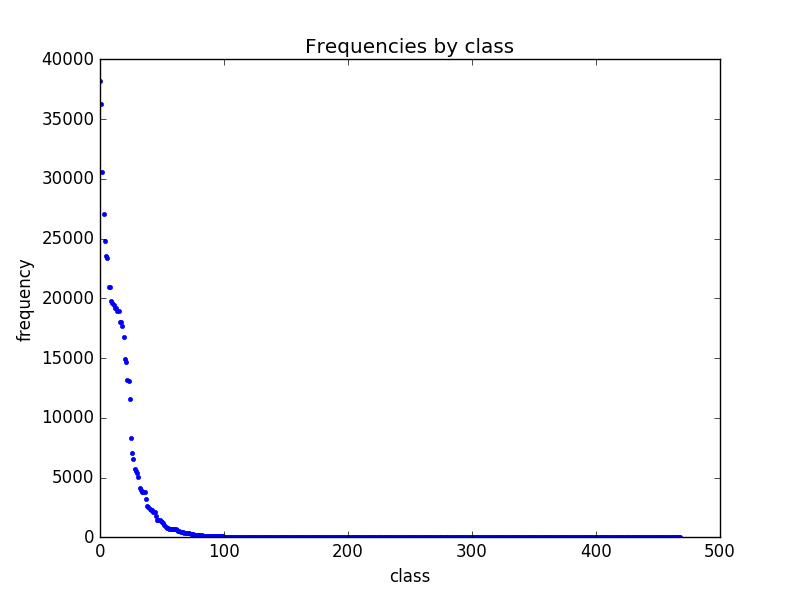
\includegraphics[width=1\textwidth]{img/dataset_frequency.png}
	\caption{Plot of frequencies for classes in \texttt{dataset}. \textit{owl:Thing} is excluded.}
	\label{fig:frequency}
\end{figure}

Step 3: Degree

The Stardog only interface handles the limits 
Python code for querying and using Stardog as endpoint. 
Query the dataset to calculate the in degree and out degree.

In degree takes 55 seconds, out degree takes 46 seconds.

\begin{lstlisting}[captionpos=b, caption=SPARQL query for calculating in degree of entities, label=lst:sparql, basicstyle=\ttfamily\small,frame=bt]
SELECT
DISTINCT ?entity
(COUNT(distinct ?pin) as ?indegree)
WHERE { 
?entity a owl:Thing .
?something ?pin ?entity .}
GROUP by ?entity
ORDER by desc(?indegree)
\end{lstlisting}

\begin{lstlisting}[captionpos=b, caption=SPARQL query for calculating out degree of entities, label=lst:sparql, basicstyle=\ttfamily\small,frame=bt]
SELECT
DISTINCT ?entity
(COUNT(distinct ?pout) as ?outdegree)
WHERE { 
?entity a owl:Thing .
?entity ?pout ?somethingelse .
}
GROUP by ?entity
ORDER by desc(?outdegree)
\end{lstlisting}

\section{Reasoning system}
Approximation by taking high quality entities. For the purpose of this paper we define the quality of an entity as its in and out degree measures. As such, when forming subgraphs based on the "smart selection" approach we take the entities in the top X\% entities.

Stardog

\section{Experimental set up}
By now we have better understanding of what the \texttt{dataset} contains. We decide to investigate information related to Amsterdam via the following query:

\begin{lstlisting}[captionpos=b, caption=SPARQL query for calculating out degree of entities, label=lst:sparql, basicstyle=\ttfamily\small,frame=bt]
SELECT distinct ?s ?p ?a
WHERE { 
?a a owl:Thing ;
rdfs:label ?la .
?s ?p ?a .
FILTER(contains(?la, 'msterdam'))
} GROUP by ?a ?s ?p
\end{lstlisting}

%TODO revise
$X$ has values of 1, 10 and 50

\section{Results and Discussion}
When ran against the whole \texttt{datset} we obtain 31 results. 

- results when random 

- results when "smart"

\section{Conclusion}
Through empirical methods, we compared the performance of two subsets of the main \texttt{dataset}. 

Weight the differences between designing an ontology or cleaning existing ontologies.

\bibliographystyle{plain}
\bibliography{mybib}

\end{document}
